\title{Lecture 10: Probability}

\frame{\titlepage}

%%%%%%%%%%%%%%%%%%
\section{Terminology}
\frame{\sectionpage}
%%%%%%%%%%%%%%%%%%

\begin{frame}
\frametitle{Random?}
\centering

\includegraphics[scale=0.5]{l04intro1.png}

\includegraphics[scale=0.5]{l04intro2.png}


\includegraphics[scale=0.5]{l04intro3.png}

\includegraphics[scale=0.15]{l04intro4.png}
\end{frame}

\begin{frame}
\frametitle{Know your vocabs}
\begin{block}{}
\begin{description}
\item[An experiment] is a planned operation carried out under controlled conditions.
\item[An outcome] is a result of an experiment.
\item[The sample space] of an experiment is the set of all possible outcomes (i.e. the universe).
\item[An event] is any combination of outcomes (i.e. a subset of the sample space).
\end{description}
\end{block}
\end{frame}


\begin{frame}[t]
\begin{ex}
Use the terminology (experiment, outcome, sample space, event) to describe rolling a single die.
\end{ex}
\begin{sol}
\begin{itemize}
\item The action of rolling a single die is an experiment.
\item An outcome could be any integer from 1 to 6.
\item The sample space is the set $\{1,2,3,4,5,6\}$
\item An event might be $\{2,4,6\}, \{1,2,3\}, \{5\}$ or $\{1,6\}$. It can even be the empty set $\phi$.
\end{itemize}
\end{sol}
\end{frame}

\begin{frame}
\frametitle{More vocabs}
\begin{block}{}
\textbf{A probability} is a \red{measure} that is associated with how certain we are of outcomes of a particular experiment or activity.
\end{block}

\begin{block}{}
The probability of any outcome is the \red{long-term relative frequency} of that outcome. It is between zero and one.
\begin{itemize}
\item The probability of zero means the event can \red{never} happen,
\item The probability of one means the event \green{always} happens,
\item The probability of one-half means the event is \blue{equally likely} to occur or not to occur.
\end{itemize}
\end{block}
\end{frame}

\begin{frame}
\addfig{0.9}{prob_defn_scale}{A probability scale from 0 to 1}{}
\end{frame}

\begin{frame}
\frametitle{Test!}
\begin{center}
{\Huge \href{https://www.menti.com/sn8imsvvw2}{Test Your Gut}}
\end{center}
\end{frame}

\begin{frame}
\frametitle{Vocabs on events}
\begin{block}{}
\begin{description}
\item[Equally likely] means that each outcome of an experiment occurs with equal probability.
\item[A fair or unbiased] randomizer (such as a dice, a coin, a card) means that all possible outcomes are equally likely.
\end{description}
\end{block}

\begin{thm}{}{}
If there are $n$ possible outcomes, and they are all equally likely, then the probability of each outcome is $\frac{1}{n}$
\end{thm}
\end{frame}

\begin{frame}
\frametitle{Mathematical Definition}
\begin{defn}{}{}
If all outcomes in the sample space are \textbf{equally likely}, then \textbf{the probability} of event $A$ is 
\begin{equation}
P(A) = \frac{|A|}{|S|}
\end{equation}
where $|A|$ is the number of elements in the set of the event $A$ and $|S|$ is the number of elements in the sample space $S$. \pause
\end{defn}
\end{frame}


\begin{frame}[t]
\begin{ex}
If we roll one fair die, what is the probability that the result is an odd number?
\end{ex}
\addfig{0.35}{l04intro1}{dice}
\begin{sol}
First, we need to start with formal definitions:
\begin{itemize}
\item The outcome can be $\epsdice[black]{1}, \epsdice[black]{2}, \epsdice[black]{3}, \epsdice[black]{4}, \epsdice[black]{5}$ or $\epsdice[black]{6}$. To simplify, let's write them as numbers 1,2,3,4,5 and 6.
\item The sample space is $\{1,2,3,4,5,6\}$
\end{itemize}
\end{sol}
\end{frame}

\begin{frame}
\begin{sol} (Continued)
\begin{itemize}
\item To find the probability, let's define the event as
\begin{center}
$A$ = the result is an odd number
\end{center}
\item By inspecting all outcomes, the event can be represented as a set $A = \{1,3,5\}$
\item Since each outcome is equally likely, the probability is
\[P(A) = \frac{|A|}{|S|} = \frac{3}{6} = \frac{1}{2}.\]
\end{itemize}
In conclusion, the probability that the result is an odd number is $\frac{1}{2}$ or $0.5$.
\end{sol}
\end{frame}

%ex


\begin{frame}[t]
\begin{ex}
If we flip two fair coins, what is the probability that at least one of them is head?
\end{ex}
\addfig{0.35}{coins_image}{Coins}
\begin{sol}
First, we need to start with formal definitions:
\begin{itemize}
\item Let a tail be $T$ and a head be $H$. Then, let's express the outcomes as a sequence of two letters. For example, $HT$ is the outcome where the first coin is head and the second coin is tail.
\item The sample space is $\{ HH, HT, TH, TT\}$. \pause
\end{itemize}
\end{sol}
\end{frame}

\begin{frame}
\begin{sol} (Continued)
\begin{itemize}
\item To find the probability, let's define the event as
\begin{center}
$B$ = at least one coin shows a head.
\end{center}
\item By inspecting all outcomes, the event can be represented as a set $B = \{HH, HT, TH\}$.
\item Since each outcome is equally likely, the probability is
\[P(B) = \frac{|B|}{|S|} = \frac{3}{4}.\]
\end{itemize}
In conclusion, the probability that at least one of them is head is $\frac{3}{4}$ or $0.75$.
\end{sol}
\end{frame}

%ex


\begin{frame}[t]
\begin{ex}
What is the probability that a random 6-digit lottery contains one digit that appears exactly 5 times? (For instance, 999997)
\end{ex}
\addfig{0.7}{rare_lottery}{\href{https://www.facebook.com/mathasitis/posts/179201643779460}{Hmmmmm}}
\end{frame}


\begin{frame}
\begin{sol}
Let $S$ be the set of all possible 6-digit lotteries. We know by the rule of product that $|S| = 10^6 = 1,000,000$.

For the specific event we are looking for, we need to use the rule of product to count. 
\begin{itemize}
\item First, choose a digit that will appear 5 times. There are 10 possible options.
\item Second, choose a digit that will be the lone digit. There are now 9 options left.
\item Finally, choose how to arrange those digits. The lone digit has 6 possible places to go, and the repeating digits will be fixed.
\end{itemize}
Because all these processes are independent, the number of lotteries with the specified pattern is $10 \times 9 \times 6 = 540$. Hence, the probability of such pattern to appear is $P(A) = \frac{|A|}{|S|} = \frac{540}{1,000,000} = 0.00054$
\end{sol}
\end{frame}

\iffalse
\begin{frame}
\begin{exercise}
Suppose you choose a random number from the set $\{1,2,3,4,5,6,7,8,9,10\}$.
\begin{enumerate}
\item What is the probability that the number is divisible by 4?
\item What is the probability that the number is greater than or equals to 5?
\item What is the probability that the number is a square?
\end{enumerate}
\end{exercise}
\end{frame}
\fi

%%%%%%%%%%%%%%%%%%
\section[Event]{Terminology for Events}
\frame{\sectionpage}
%%%%%%%%%%%%%%%%%%

\begin{frame}
\frametitle{Or}
\begin{block}{}
\begin{description}
\item[$A$ or $B$] An outcome is in the event ``$A$ or $B$'' if the outcome is in the set $A \cup B$. In other words, it is in A or is in B or is in both A and B.
\end{description}
\end{block}
\begin{figure}[h!]
\centering
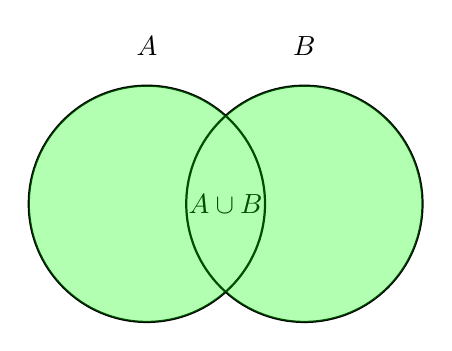
\begin{tikzpicture}[thick]
\draw (0,0) circle (15mm);
\draw (2,0) circle (15mm);
\node at (0,2) {$A$}; 
\node at (2,2) {$B$};
\node at (1,0) {$A \cup B$};
\fill[green, fill opacity = 0.3] (2,0)  circle (15mm) (0,0)  circle (15mm);
\end{tikzpicture}
\caption{Venn diagram for $A$ or $B$}
\end{figure}
\end{frame}

\begin{frame}
\frametitle{And}
\begin{block}{}
\begin{description}
\item[$A$ and $B$] An outcome is in the event ``$A$ and $B$'' if the outcome is in the set $A \cap B$. In other words, it is in A or is in B or is in both A and B.
\end{description}
\end{block}
\begin{figure}[h!]
\centering
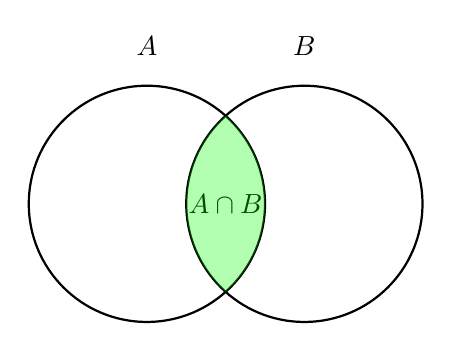
\begin{tikzpicture}[thick]
\draw (0,0) circle (15mm);
\draw (2,0) circle (15mm);
\node at (0,2) {$A$}; 
\node at (2,2) {$B$};
\node at (1,0) {$A \cap B$};
  \clip (0, 0)  circle (15mm);
  \fill[green, fill opacity = 0.3] (2,0)  circle (15mm);
\end{tikzpicture}
\caption{Venn diagram for $A$ and $B$}
\end{figure}
\end{frame}


\begin{frame}[t]
\begin{ex}
Suppose we roll one fair dice. 
\begin{enumerate}
\item Find the probability of getting an odd number \textbf{or} a number higher than 3.
\item Find the probability of getting an odd number \textbf{and} a number higher than 3.
\end{enumerate}
\end{ex}
\addfig{0.4}{dice_monster}{Cute...?}
\end{frame}


\begin{frame}[t]
\begin{sol}
Let $A$ = get an odd number, and $B$ = get a number higher than 3. We can express them as sets
\[A = \{1,3,5\} \qquad B = \{4,5,6\}.\]
This gives us the following Venn diagram.
\begin{figure}[h!]
\centering
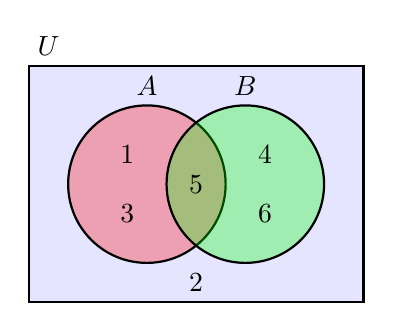
\begin{tikzpicture}[thick, scale=0.5]
\node at (-2.5,3.5) {$U$};
\filldraw[fill = blue, fill opacity = 0.1] (-3,-3) rectangle (5.5,3);
\node at (0,2.5) {$A$};
\node at (2.5,2.5) {$B$};
  \filldraw[fill=red, fill opacity = 0.3]  (0,0)    circle (20mm);
  \filldraw[fill=green, fill opacity = 0.3] (2.5,0)  circle (20mm);
  \node at (1.25,0) {5};
  \node at (-0.5, 0.75) {1};
  \node at (-0.5, -0.75) {3};
  \node at (3, 0.75) {4};
  \node at (3, -0.75) {6};
  \node at (1.25, -2.5) {2};
\end{tikzpicture}
\caption{Venn diagram for $A$ and $B$}
\end{figure}
\end{sol}
\end{frame}

\begin{frame}[t]
\begin{sol}
In terms of sets, we have
\[A \cup B = \{1,3,4,5,6\} \text{  and  } A \cap B = \{5\}\]
\begin{enumerate}
\item This is equivalent to $P(A \text{or} B)$, so we have $P(A \cup B) = \frac{|A \cup B|}{|S|} = \frac{5}{6}$.
\item This is equivalent to $P(A \text{ and }B)$, so we have $P(A \cap B) = \frac{|A \cap B|}{|S|} = \frac{1}{6}$. Likewise, we can deduce that the only outcome that is odd and higher than 3 is 5, so we immediately get the probability of $\frac{1}{6}$.
\end{enumerate}
\end{sol}
\end{frame}

\begin{frame}
\frametitle{Mutually Exclusive}
\begin{block}{}
\begin{description}
\item[Mutually exclusive] If $A \cap B = \{\}$, we say that $A$ and $B$ are \red{mutually exclusive}.
\end{description}
\end{block}
\begin{figure}[h!]
\centering
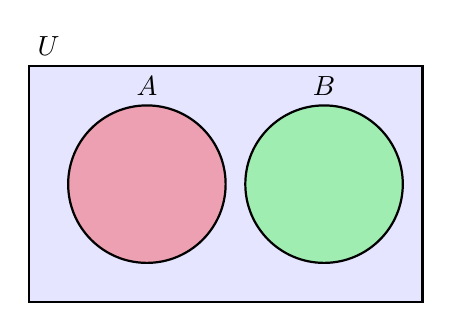
\begin{tikzpicture}[thick, scale=0.5]
\node at (-2.5,3.5) {$U$};
\filldraw[fill = blue, fill opacity = 0.1] (-3,-3) rectangle (7,3);
\node at (0,2.5) {$A$};
\node at (4.5,2.5) {$B$};
  \filldraw[fill=red, fill opacity = 0.3]  (0,0)    circle (20mm);
  \filldraw[fill=green, fill opacity = 0.3] (4.5,0)  circle (20mm);
  \end{tikzpicture}
\caption{$A$ are $B$ mutually exclusive.}
\end{figure}
\end{frame}

 
\begin{frame}[t] 
\begin{ex} 
Suppose we roll two fair dice. Find all pairs of events below that are mutually exclusive.
\begin{itemize}
\item $A$ = the sum of both dice is 8
\item $B$ = both dice have the same value
\item $C$ = first dice is 1
\item $D$ = the difference of both dice is 3
\end{itemize}
\end{ex} 
\addfig{0.35}{two_dice}{Two Dice}
\end{frame}

\begin{frame}
\begin{sol}
We see that
\begin{itemize}
\item $A$ and $D$ are mutually exclusive. You can tell without listing all the elements because if both dice have the same value, then the different must be 0, not 3. 
\item On the other hand, $A \cap B = \{11\}$ and $A \cap C = \{44\}$, so neither pair $A$ and $B$, or $A$ and $C$ are mutually exclusive.
\item $B$ and $C$ are mutually exclusive. If the first dice is 1 and the sum is 8, then the other dice would need to be 7.
\item $C$ and $D$ are mutually exclusive. Again, we can see algebraically that if the sum is 8, then both numbers are even or odd, so the difference will always be even.
\end{itemize}

\end{sol}
\end{frame}

\begin{frame}
Alternatively, we can express the events as sets and use Venn diagram.
\begin{eq*}
A &=& \{26, 35, 44, 53, 62\} \\
B &=& \{11, 22, 33, 44, 55, 66\} \\
C &=& \{11, 12, 13, 14, 15 ,16\} \\
D &=& \{14, 25, 36, 41, 52, 63\}
\end{eq*}
\begin{figure}[h!]
\centering
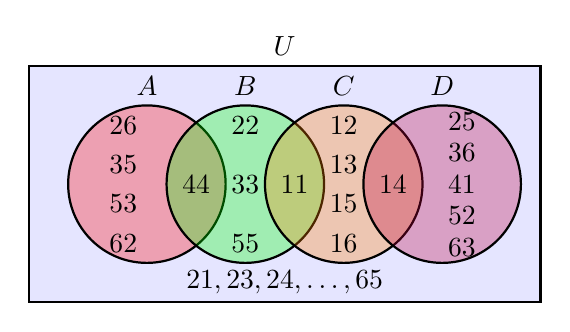
\begin{tikzpicture}[thick, scale=0.5]
\node at (3.5,3.5) {$U$};
\filldraw[fill = blue, fill opacity = 0.1] (-3,-3) rectangle (10,3);
\node at (0,2.5) {$A$};
\node at (2.5,2.5) {$B$};
\node at (5,2.5) {$C$};
\node at (7.5,2.5) {$D$};
  \filldraw[fill=red, fill opacity = 0.3]  (0,0)    circle (20mm);
  \filldraw[fill=green, fill opacity = 0.3] (2.5,0)  circle (20mm);
  \filldraw[fill=orange, fill opacity = 0.3] (5,0)  circle (20mm);
  \filldraw[fill=purple, fill opacity = 0.3] (7.5,0)  circle (20mm);
\node at (1.25,0) {44};
\node at (3.75,0) {11};
\node at (6.25,0) {14};
\node at (-0.6,1.5) {26};
\node at (-0.6,0.5) {35};
\node at (-0.6,-0.5) {53};
\node at (-0.6,-1.5) {62};
\node at (2.5,1.5) {22};
\node at (2.5,0) {33};
\node at (2.5,-1.5) {55};
\node at (5,1.5) {12};
\node at (5,0.5) {13};
\node at (5,-0.5) {15};
\node at (5,-1.5) {16};
\node at (8,1.6) {25};
\node at (8,0.8) {36};
\node at (8,0) {41};
\node at (8,-0.8) {52};
\node at (8,-1.6) {63};
\node at (3.5, -2.5) {$21, 23, 24, \ldots, 65$};
\end{tikzpicture}
\caption{Venn diagram for $A,B,C$ and $D$}
\end{figure}
\end{frame}

\iffalse
\begin{frame}
\begin{exercise}
Suppose we roll two fair dice. Find all pairs of events below that are mutually exclusive.
\begin{itemize}
\item $A$ = both dice have the same value
\item $B$ = first dice is 2
\item $C$ = the sum of both dice is 9
\item $D$ = the difference of both dice is 4
\end{itemize}
\end{exercise}
\end{frame}
\fi

%%%%%%%%%%%%%%%%%%
\section[Conditional]{Conditional Probability}
\frame{\sectionpage}
%%%%%%%%%%%%%%%%%%

\begin{frame}
\frametitle{Conditional Probability}

\begin{block}{}
\begin{description}
\item[$P(A | B)$] The \red{conditional probability} of A given B is the probability that event A will occur given that the event B has already occurred

\item A conditional \textbf{reduces} the sample space. For $P(A|B)$, we look at the sample space $B$, and see all outcomes that are also in $A$.
\end{description}
\end{block}
Note: $A|B$ itself has no meaning as a set or a probability. We always see it as $P(A|B)$.

\frametitle{Formula for Conditional Probability}
\begin{defn}{}{}
If $B$ is not an empty set, then we define
\begin{equation}
P(A|B) = \frac{P(A \cap B)}{P(B)}
\end{equation}
\end{defn}
\end{frame}



\begin{frame}
\frametitle{}
\begin{figure}[h!]
\centering
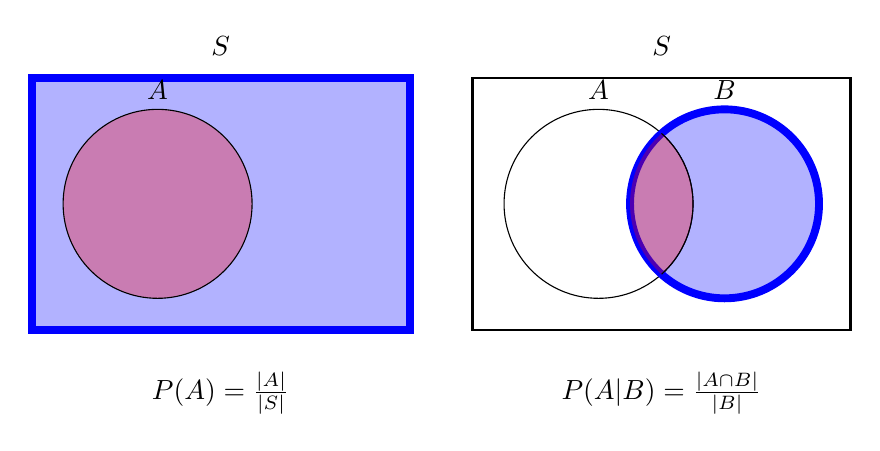
\begin{tikzpicture}[scale=0.8]
\filldraw[fill=blue, fill opacity = 0.3, line width = 1mm, color = blue] (0,0) rectangle (6,4);
\filldraw[fill=red, fill opacity = 0.3]  (2,2)    circle (15mm);
\node at (2,3.8) {$A$};
\node at (3,4.5) {$S$};
\node at (3,-1) {$P(A) = \frac{|\red{A}|}{|\blue{S}|}$};
\begin{scope}[xshift=7cm]
\draw[thick] (0,0) rectangle (6,4);
\draw (2,2) circle (15mm);
\node at (3,4.5) {$S$};
\node at (2,3.8) {$A$};
\node at (4,3.8) {$B$};
\node at (3,-1) {$P(A|B) = \frac{|\red{A \cap B}|}{|\blue{B}|}$};
\filldraw[fill=blue, color = blue, line width = 1mm, fill opacity = 0.3] (4,2)  circle (15mm);
\clip (4,2) circle (15mm);
\filldraw[fill=red, fill opacity = 0.3]  (2,2) circle (15mm);
\end{scope}
\end{tikzpicture}
\caption{Comparing $P(A)$ to $P(A|B)$}
\end{figure}
\end{frame}


\begin{frame}[t]
\begin{ex}
Suppose we roll one fair die. 
\begin{enumerate}
\item Find the probability of getting an even number, \textbf{given} that it is higher than 2.
\item Find the probability of getting a number higher than 2, \textbf{given} that it is even.
\end{enumerate}
\end{ex}
\addfig{0.2}{dice_devil_head}{Fair, sure....}{}
\end{frame}

\begin{frame}[t]
\begin{sol}
Let $A$ = get an even number, and $B$ = get a number higher than 2. We can express them as sets
\[A = \{2,4,6\} \qquad B = \{3, 4,5,6\}\]
This gives us
\[ A \cap B = \{4,6\}\]
\begin{enumerate}
\item This is equivalent to $P(A| B) = \frac{P(A \cap B)}{P(B)} = \frac{2/6}{4/6} = \frac{1}{2}$
\item This is equivalent to $P(B|A) = \frac{P(B \cap A)}{P(A)} = \frac{2/6}{3/6} = \frac{2}{3}$
\end{enumerate}
Notice that these two probabilities are different, so the order matters.
\end{sol}
\end{frame}

\begin{frame}
\frametitle{}
\begin{figure}[h!]
\centering
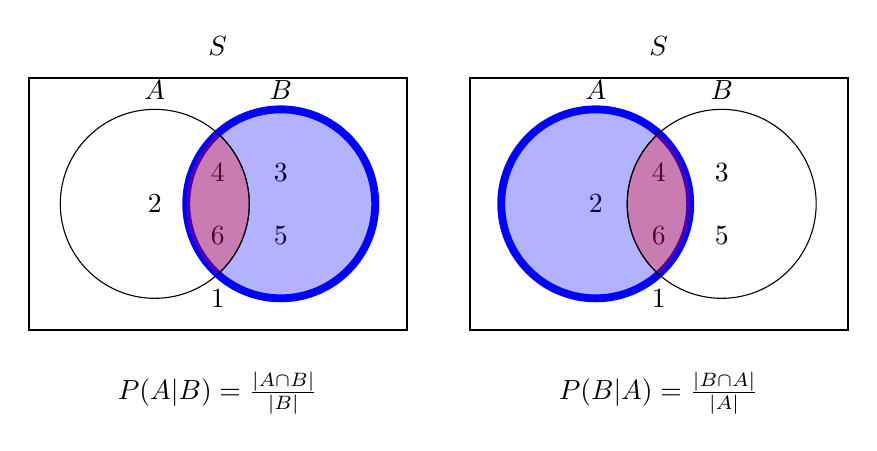
\begin{tikzpicture}[scale=0.8]
\begin{scope}
\draw[thick] (0,0) rectangle (6,4);
\node at (3,4.5) {$S$};
\node at (2,3.8) {$A$};
\node at (4,3.8) {$B$};
\node at (3,0.5) {1};
\node at (2,2) {2};
\node at (3,2.5) {4};
\node at (3,1.5) {6};
\node at (4,2.5) {3};
\node at (4,1.5) {5};
\node at (3,-1) {$P(A|B) = \frac{|\red{A \cap B}|}{|\blue{B}|}$};
\draw (2,2) circle (15mm);
\filldraw[fill=blue, fill opacity = 0.3, line width = 1mm, color = blue] (4,2)  circle (15mm);
\clip (4,2) circle (15mm);
\filldraw[fill=red, fill opacity = 0.3]  (2,2) circle (15mm);
\end{scope}
\begin{scope}[xshift=7cm]
\draw[thick] (0,0) rectangle (6,4);
\node at (3,4.5) {$S$};
\node at (2,3.8) {$A$};
\node at (4,3.8) {$B$};
\node at (3,0.5) {1};
\node at (2,2) {2};
\node at (3,2.5) {4};
\node at (3,1.5) {6};
\node at (4,2.5) {3};
\node at (4,1.5) {5};
\node at (3,-1) {$P(B|A) = \frac{|\red{B \cap A}|}{|\blue{A}|}$};
\filldraw[fill=blue, fill opacity = 0.3, line width = 1mm, color = blue] (2,2)  circle (15mm);
\draw (4,2) circle (15mm);
\clip (2,2) circle (15mm);
\filldraw[fill=red, fill opacity = 0.3]  (4,2) circle (15mm);
\end{scope}
\end{tikzpicture}
\caption{Venn diagrams to compute $P(A|B)$ and $P(B|A)$}
\end{figure}
\end{frame}

 
\begin{frame}[t] 
\begin{ex} 
A family has two kids, each is equally likely to be male or female. Suppose we know that one of them is male. Find the probability of the following events.
\begin{tasks}(1)
\task $A_1$ = they are both female.
\task $A_2$ = they are both male.
\end{tasks}
\end{ex} 
\addfig{0.4}{two_children_paradox}{Happy Family}
\end{frame}


\begin{frame}[t] 
\begin{sol}
Denote $F$ as female and $M$ as male. Then, we can express all possibilities as $S = \{MM, MF, FM, FF\}$. We also have  
\[A_1 = \{FF\} \quad \text{ and } \quad A_2 = \{MM\}.\]

\medskip
Let $B$ = one of the kids is male. Then, we can see that 
\[B = \{FM, MF, MM\}.\]
\begin{tasks}(1)
\task It is clear from the sentence that they cannot both be female, as one of them is known to be male. Thus, we immediately conclude that $P(A_1|B) = 0$.
\task Using the formula, we get $P(A_2 |B) = \frac{P(A_2 \cap B)}{P(B)} = \frac{1/4}{3/4} = \frac{1}{3}$
\end{tasks}
\end{sol}
\end{frame}

\iffalse
\begin{frame}
\begin{exercise}
Suppose we roll two fair dice, one after another.
\begin{enumerate}
\item Find the probability that the sum is greater than 7, given that the first die is less than 3.
\item Find the probability that the first die is less than 3, given that the sum is greater than 7.
\item Find the probability that the sum is odd, given that the dice have the same value.
\end{enumerate}
\end{exercise}
\end{frame}
\fi

%%%%%%%%%%%%%%%%%%
\section[Basic rules]{Basic rules for probability}
\frame{\sectionpage}
%%%%%%%%%%%%%%%%%%

\begin{frame}
\frametitle{Basic properties for probability}
Instead of having to determine the sample space and the set of outcomes every time, we can use some properties and rules to help us.
\begin{thm}{}{}
For any event $A$ in the sample space $S$, the followings are true:
\begin{itemize}
\item $0 \leq P(A) \leq 1$  \pause
\item $P(A^c) + P(A) = 1$. Recall that $A^c$ is the complement of $A$. \pause
\item $P(A \cup B) = P(A) + P(B) - P(A \cap B)$
\end{itemize}
\end{thm}
Note that the third property is also known as inclusion-exclusion principle in counting principles.
\end{frame}

 
\begin{frame}[t] 
\begin{ex} 
What is the probability of flipping 6 coins and getting at least 2 heads?
\end{ex} 
\begin{sol}
Let $A$ = at least one coin shows a head. Lots of outcomes are in $A$, for example $HHTTHH, HTTTHH, \ldots$, so it might be better to look for $A^c$. The complement of $A$ is the set of outcomes where there are \textbf{at most} 1 head, so either 0 heads or 1 head. Here, we can easily see that 
\begin{eq*} 
A^c &=& \{TTTTTT, HTTTTT, THTTTT, TTHTTT, \\
&\qquad& TTTHTT, TTTTHT, TTTTTH\}
\end{eq*}
Now we have $P(A^c) = \frac{|A|}{|S|} = \frac{7}{2^6} = \frac{7}{64}$. Thus, we have $P(A) = 1- P(A^c) = 1 - \frac{7}{64} = \frac{57}{64}$.
\end{sol}
\end{frame}

 
\begin{frame}[t]
\begin{ex} 
 Let $S$ be the set of standard deck of cards $\{A\heartsuit, A\diamondsuit, A\spadesuit, A\clubsuit, 2\heartsuit, \ldots, K\clubsuit\}$. \pause What is the probability of drawing a card that is either an ace \textbf{or} a heart.
\end{ex} 
\begin{sol}
Let $A$ = the event of drawing an ace, and $\heartsuit$ = the event of drawing a heart. We know that 
\begin{itemize}
\item Since there are 4 aces in the deck, we have $P(A) = \frac{4}{52}$.
\item Since there are 13 hearts in the deck, $P(\heartsuit) = \frac{13}{52}$. \pause
\item Since there is only 1 card that is both and ace and a heart (namely $A\heartsuit$), $P(A \cap \heartsuit) = \frac{1}{52}$
\end{itemize}
Therefore, the probability of getting an ace or a heart, namely $A \cup B$, is
\[P(A \cup B) = P(A) + P(B) - P(A \cap B) = \frac{4}{52} + \frac{13}{52} - \frac{1}{52} = \frac{16}{52}\]
\end{sol}
\end{frame}


\begin{frame}
\frametitle{The Multiplication Rule}
The rule of addition for counting principles can be translated to a probability term as follows.
\begin{defn}{}{}
Events $A$ and $B$ are \red{independent} if the knowledge that one occurred does not affect the chance the other occurs. Formally, $A$ and $B$ are independent if and only if we have $P(A|B) = P(A).$
\end{defn}
\end{frame}

\begin{frame}[t]
\begin{ex}
Determine whether each pair of events are independent or not.
\begin{tasks}(1)
\task The event that a fair coin lands heads, and the event that a fair die rolls a 5.
\task The event that a card is a king, and the event that a card is a club.
\end{tasks}
\end{ex}
\begin{sol}
\begin{tasks}(1)
\task Yes. Two separate experiments do not affect each other.
\task Yes. 
\end{tasks}
\end{sol}
\end{frame}


\begin{frame}[t]
\begin{ex}
Determine whether each pair of events are independent or not.
\begin{tasks}(1)
\task The event that the top card of a shuffled deck of cards is red, and the event that the bottom card is black.
\task The event that the first 49 coin flips are tails, and the 50th coin flip is also a tail.
\end{tasks}
\end{ex}
\begin{sol}
\begin{tasks}(1)
\task No. Suppose you know that the top card is red. Then, the rest of the deck will have 25 red cards and 26 black cards, so the probability becomes $\frac{25}{51}$.
\task Yes. The information of previous flips do not affect the next flip.
\end{tasks}
\end{sol}
\end{frame}

\begin{frame}[t]
\begin{thm}{}{}
Events $A$ and $B$ are \textbf{independent} if and only if
\begin{equation}
P(A \cap B) = P(A) P(B)
\end{equation}
\end{thm}
\begin{proof}
Since we are given that $P(A|B) = P(A)$ and we know that $P(A|B) = \frac{P(A\cap B)}{P(B)}$, we have
\begin{eq*}
P(A) &= \frac{P(A\cap B)}{P(B)} \\
P(A\cap B) &= P(A) P(B)
\end{eq*}
\end{proof}
\end{frame}

\begin{frame}[t]
\begin{ex}
Suppose you roll a six-sided die. Let $A$ be the event that the roll is even, and $B$ be the event that the roll is greather than or equal to 5. Prove whether $A$ and $B$ are independent 
\end{ex}
\begin{sol}
We can write $A = \{2,4,6\}$ and $B  \{5,6\}$, so $P(A) = \frac{3}{6}$ and $P(B) = \frac{2}{6}$. Therefore, the product is $P(A) P(B) = \left( \frac{3}{6} \right) \left( \frac{2}{6} \right) = \frac{1}{6}$.
\medskip

We can see that $A \cap B = \{6\}$ (or that 6 is the only even result which is also greather than or equal to 5), so $P(A \cap B) = \frac{1}{6}$. Thus, we have

\[P(A \cap B) = \frac{1}{6} = P(A)P(B).\]

Therefore, we conclude that $A$ and $B$ are independent.
\end{sol}
\end{frame}

 
\begin{frame}[t]
\begin{ex} 
Suppose we roll 3 fair dice. What is the probability that each of them shows at least 5.
\end{ex} 
\begin{sol}
From now on, we will assume that dice results are independent.
\medskip
 
 Let $A_1$ = the first dice showing at least 5, $A_2$ = the second dice showing at least $5$, and $A_3$ = the third dice showing at least $5$. We see that $P(A_1) = P(A_2) = P(A_3) = \frac{2}{6}$. 

\medskip Therefore, the probability of getting all numbers at least 5 is $P_1 \cap P_2 \cap P_3$, which gives
\[P(A_1 \cap A_2 \cap A_3) = P(A_1) P(A_2) P(A_3) = \frac{2}{6} \times \frac{2}{6} \times \frac{2}{6} = \frac{1}{27}\]
\end{sol}
\end{frame}

\begin{frame}
\frametitle{The Addition Rule}
The rule of addition for counting principles can also be translated to a probability term.
\begin{thm}{}{}
If events $A$ and $B$ are \textbf{mutually exclusive} (i.e. $A \cap B = \{\}$), then we have
\begin{equation}
P(A \cup B) = P(A) + P(B)
\end{equation}
\end{thm}
This is simply division into several cases, where each case is different. The theorem emphasizes the word ``mutually exclusive''.
\end{frame}

 
\begin{frame}[t]
\begin{ex} 
Suppose there are 9 players in a match of Among Us, with 5 Asians and 4 Americans. If two players are randomly selected as impostors with equal chance, what is the probability that they share the same race?
\end{ex} 
\addfig{0.6}{among_us}{Everyone else smells like a traitor.}
\end{frame}

\begin{frame}[t]
\begin{sol}
Let $A$ = both players are Asians and $B$ = both players are Americans. Since we don't care about the order, this is a problem about combination.
\begin{itemize}
\item If there is no restriction, the number of combinations of two players is $C(9,2) = \frac{9!}{7!2!} = 36$. Thus, $|S| = 36$. 
\item If they are both Asians, then the number of combinations is $C(5,2) = \frac{5!}{3!2!} = 10$. Thus, $P(A) = \frac{10}{36}$
\item If they are both Americans, the number of combinations is $C(4,2) = \frac{4!}{2!2!} = 6$. Thus, $P(B) = \frac{6}{36}$

Since both events are mutually exclusive, the probability that either event occurs is
\[ P(A \cup B) = P(A) + P(B) = \frac{10}{36} + \frac{6}{36} = \frac{16}{36} = \frac{4}{9}\]
\end{itemize}
\end{sol}
\end{frame}

\iffalse
\begin{frame}
\begin{exercise}
Suppose that you have eight cards. Five are green and three are yellow. The five green cards are numbered 1, 2, 3, 4, and 5. The three yellow cards are numbered 1, 2, and 3. The cards are well shuffled. You randomly draw one card.
\medskip

Let $G$ be the event where the card drawn is green, and $E$ be the event where the card drawn is even.
\begin{enumerate}
\item List the sample space.
\item Find $P(G), P(G|E), P(G \cap E), P(G \cup E)$.
\item Are G and E mutually exclusive? Justify your answer numerically.
\end{enumerate}
\end{exercise}
\end{frame}
\fi